% !TEX root = ../thesis.tex

\chapter{Analýza štruktúry genómu a nástrojov na jej reprezentáciu}

Táto kapitola sa venuje analýze štruktúry genómu rôznych organizmov, alebo inými slovami biologickému pozadiu, ktoré je nevyhnutné pre vytvorenie akéhokoľvek bioinformatického softvéru.
Lebo bez pochopenia toho, ako je organizovaný genóm, nedá sa aj navrhunuť nástroj na jeho vizualizáciu.

Okrem toho, táto kapitola osobitne popisuje a porovnáva existujúce riešenia pre reprezentáciu údajov o genóme s cieľom porozumieť moderným prístupom k vizualizácii štruktúry genómu. 

Každá zo spomínaných tém je popísaná v zodpovedajúcej podsekcii.

\section{Všeobecná štruktúra genómu}
U väčšiny organizmov je dedičným materiálom buď lineárna dvojvláknová molekula DNA (deoxyribonukleová kyselina) alebo kruhová dvojvláknová molekula DNA.
Avšak, niektoré extracelulárne formy života môžu používať RNA (ribonukleová kyselina) ako stavebný blok svojho genómu.
Napríklad vírusy majú genóm zložený buď z jednovláknovej DNA, dvojvláknovej DNA alebo RNA, v závislosti od typu vírusu.

Samotný genóm teda je úplná genetická informácia, alebo inými slovami, všetky jedinečné sekvencie DNA (RNA) organizmu.

%%%%%%%%%%%%%%%%%%%%%%%%%%%%%%%%%%%%%%%%%%%%%%%%%%%%%%
\subsection{Nukleotidy: základná podjednotka genómu}
%%%%%%%%%%%%%%%%%%%%%%%%%%%%%%%%%%%%%%%%%%%%%%%%%%%%%%
DNA aj RNA sú polymérové molekuly, ktoré sú zložené z lineárnych reťazcov rôznych kombinácií štyroch typov nukleotidov.

Samotný nukleotid je základnou jednotkou molekúl DNA a RNA, monomérom, ktorý sa však v bunke nachádza nielen ako nosič genetickej informácie,
ale tiež ako nosič energie použitej na napájanie enzymatických reakcií \cite{AnalysisOfGenesAndGenomes}. 

Cukor s piatimi atómami uhlíka, fosfátová skupina a dusíkatá zásada sú tri odlišné zložky, ktoré spolu tvoria celkom zložitú molekulu nukleotidov.
Kombinácia cukru a bázy sa nazýva nukleozid, zatiaľ čo fosfát-cukor-báza sa nazýva nukleotid. 

Nukleotidom môže byť buď purín s dvojitým kruhom, alebo pyrimidín s jedným kruhom (obr. 1.2).
Guanín (G) a adenín (A) sú bežné puríny pre DNA aj RNA; pyrimidín nazývaný cytozín (C) je tiež prítomný v obidvoch nukleových kyselinách.
Pyrimidín uracil (U) je však obmedzený iba na RNA, ktorý je v DNA nahradený tymínom (T).

Sú prípustné iba dve kombinácie párov báz - A párovaný s T (U) a C párovaný s G (obr. 1.1).
Stáva sa to kvôli geometriám nukleotidových báz a relatívnym pozíciám atómov, ktoré sa podieľajú na spojení \cite{MolecularGenetics}.
Táto vlastnosť robí dve sekvencie polynukleotidov v skrutkovnicie DNA (RNA) komplementárnymi. 

\begin{figure}[!ht]
	\centering
	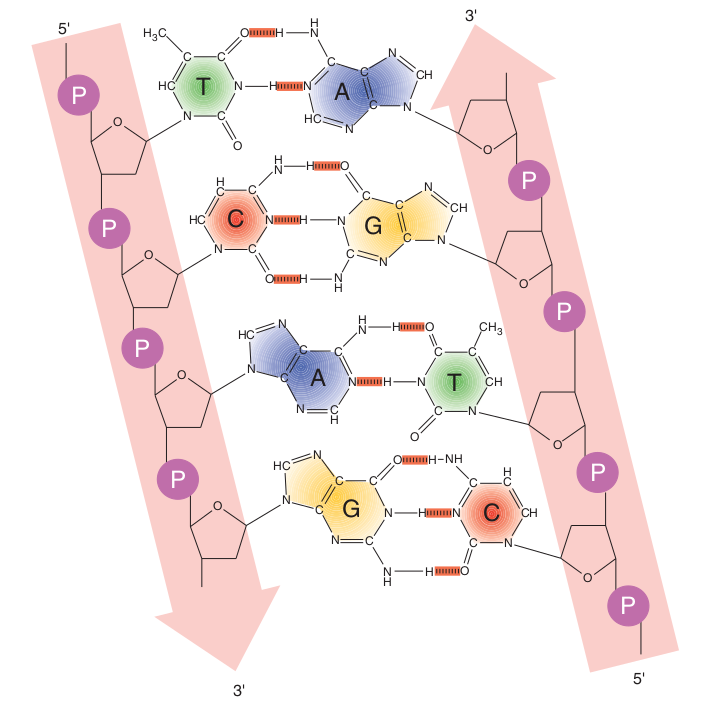
\includegraphics[width=.85\textwidth]{figures/nucleotides.png}
	\caption{Párovanie a komplementácia báz DNA. Dva reťazce skrutkovice, ktoré sú šípené v smere 5` až 3`, sú antiparalelné. Základne na jednom vlákne špirály
	sú komplementárne k tým na opačnom vlákne, A vždy párovaný s T a G vždy párovaný s C \label{o:nucleotide}}
\end{figure}

\begin{figure}[!ht]
	\centering
	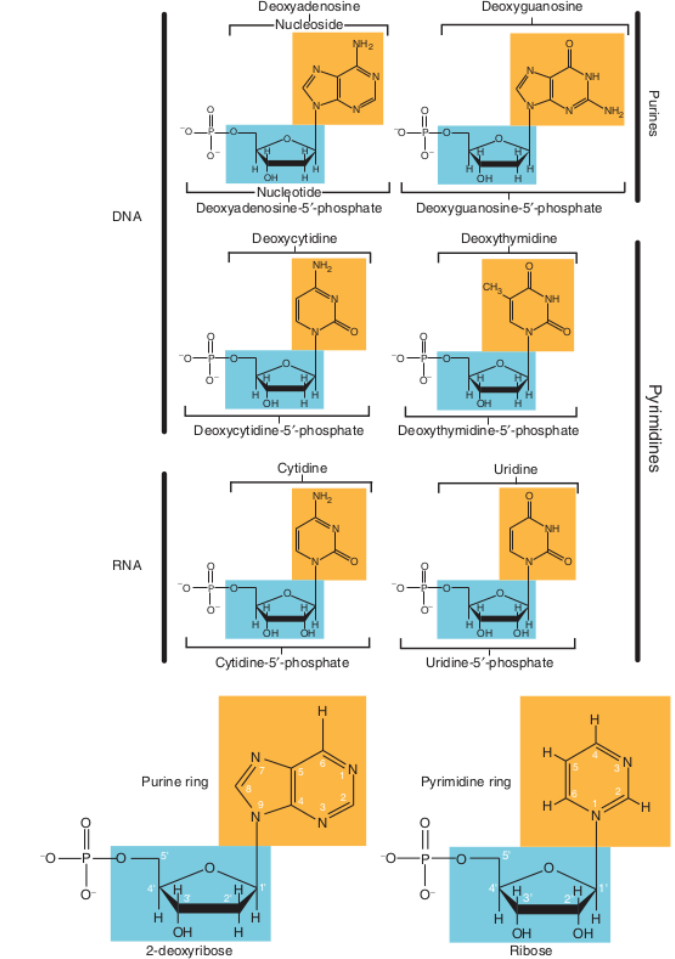
\includegraphics[width=.9\textwidth]{figures/bases1.png}
	\caption{Štruktúry nukleotidov nachádzajúcich sa v DNA a RNA. Skupiny cukru sú zvýraznené modrou farbou a dusíkaté zásady sú zvýraznené oranžovou farbou.
	Atómy cukru sú očíslované od 1 do 5. Atómy purínového kruhu sú očíslované od 1 do 9, zatiaľ čo tie pyrimidínového kruhu sú očíslované od 1 do 6. \label{o:nucleotides}}
\end{figure}

Dinukleotid, trinukleotid a polynukleotid sú výrazy zodpovedajúce dvom, trom alebo mnohým nukleotidom spojených navzájom.

Každý koniec molekuly DNA je označený číslom: jeden koniec sa označuje ako 5') a druhý koniec sa označuje ako 3'. 
Čísla 5' a 3' označujú počet atómov uhlíka v molekule cukru deoxyribózy, ku ktorým sa viaže fosfátová skupina.

Diskrétne nukleotidy sú navzájom spojené cukrom-fosfátovými väzbami, ktoré spájajú fosfátovú skupinu na 5' uhlíku jedného nukleotidu s hydroxylovou skupinou na 3' uhlíku iného nukleotidu.
Párovanie báz medzi adenínom a tymínom (uracil) zahŕňa dve vodíkové väzby, ale medzi cytozínom a guanínom tri vodíkové väzby. 

%%%%%%%%%%%%%%%%%%%%%%%%%%%%%%%%%%%%%%%%%%%%%
\subsection{Priestorová štruktúra nukleovej kyseliny}
%%%%%%%%%%%%%%%%%%%%%%%%%%%%%%%%%%%%%%%%%%%%%
Pretože trojrozmerná štruktúra nukleotidu nie je úplne tuhá, je možné, aby DNA mala rôzne priestorové architektúry:
A-forma, B-forma, Z-forma a kruhová (tab. 1.1). Poloha bázy vzhľadom na cukor s piatimi atómami uhlíka sa môže meniť rotáciou
a týmto spôsobom významne ovplyvňujú trojrozmernú konfiguráciu molekuly a skrutkovice následne, ktorá je viditeľna na obrázku 1.3.
\begin{table}[!ht]
	\caption{Dvojvláknová špirála DNA}\label{t:1}
	\smallskip
	\centering
	
	\begin{tabular}{ |p{3cm}||p{3cm}|p{3cm}|p{3cm}|  }
		\hline
		\multicolumn{4}{|c|}{Vlastnosti rôznych konformácií dvojitej špirály DNA} \\
		\hline
		Vlastnosť& B-forma & A-forma & Z-forma\\
		\hline
		\hline
		Typ špirály & Pravotočivá & Pravotočivá & Ľavotočivá \\
		\hline
		Počet párov báz na ťah & 10 & 11 & 12\\
		\hline
		Vzdialenosť medzi pármi báz (nm) & 0.34 & 0.29 & 0.37\\
		\hline
		Vzdialenosť na jedno otočenie (nm) & 3.4 & 3.2 & 4.5\\
		\hline
		Priemer (nm) & 2.37 & 2.55 & 1.84\\
		\hline
		Hlavná drážka & Široká, hlboká & Úzka, hlboká & Plochá\\
		\hline
		Vedľajšia drážka & Úzka, plytká & Široká plytká & Úzka, hlboká\\
		\hline
	\end{tabular}
\end{table}

\begin{figure}[!ht]
	\centering
	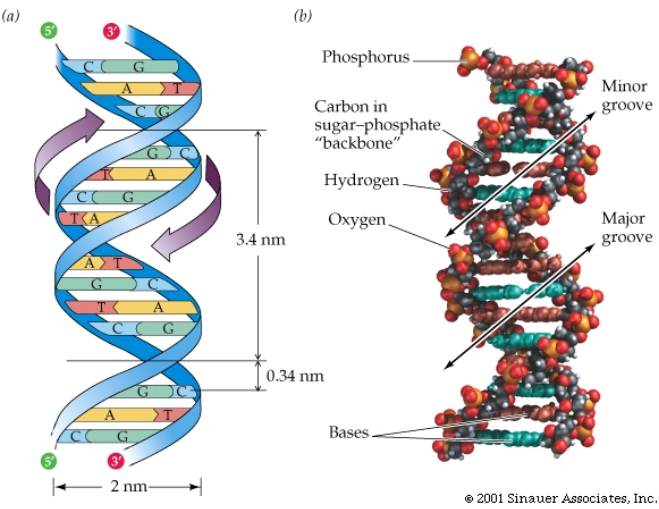
\includegraphics[width=.85\textwidth]{figures/spatial.png}
	\caption{Dvojvláknová špirála DNA.\label{o:latex_friendly_zone}}
\end{figure}

Aj keď sú RNA zvyčajne jednoreťazcové, niektoré sekvencií sú schopne tvoriť dvojité špirály.
Dvojité špirály RNA sú však zriedkavé a nezdá sa, že sa podieľajú na procesoch súvisiacich s genómom v eukaryotických a prokaryotických organizmoch.
Naviac, kruhová DNA môže existovať v niekoľkých formách, vrátane jednostrannej C-DNA, intaktnej dvojvláknovej C-DNA (uzavreté kruhy s oboma prameňmi kovalentne spojené),
prezývaná DS-C-DNA (iba jeden prameň kovalentne spojený) a vo forme "zreťazených kruhov" \cite{MolecularGenetics}, ale ich vlastnosti nie sú opísané v priloženej tabuľke 1.1 .

%%%%%%%%%%%%%%%%%%%%%%%%%%%%%%%%%%%%%%%%%%%%
\subsection{Organizácia eukaryotického genómu}
%%%%%%%%%%%%%%%%%%%%%%%%%%%%%%%%%%%%%%%%%%%%
Eukaryoty sú organizmy, ktorých bunky majú jadro uzavreté v jadrovom obale \cite{BioDict}.
V eukaryotických bunkách sa nukleová kyselina nachádza v organele viazanej na membránu, ktorá sa nazýva jadro.

Jadrový genóm je rozdelený na súbor lineárnych molekúl DNA s dvojitou špirálou, z ktorých každá je obsiahnutá v chromozóme.
Samotný chromozóm je lineárny reťazec DNA obalený okolo asociovaných proteínov, ktoré dávajú štruktúru spojenej s nimi nukleovéj kyseline.

\begin{figure}[!ht]
	\centering
	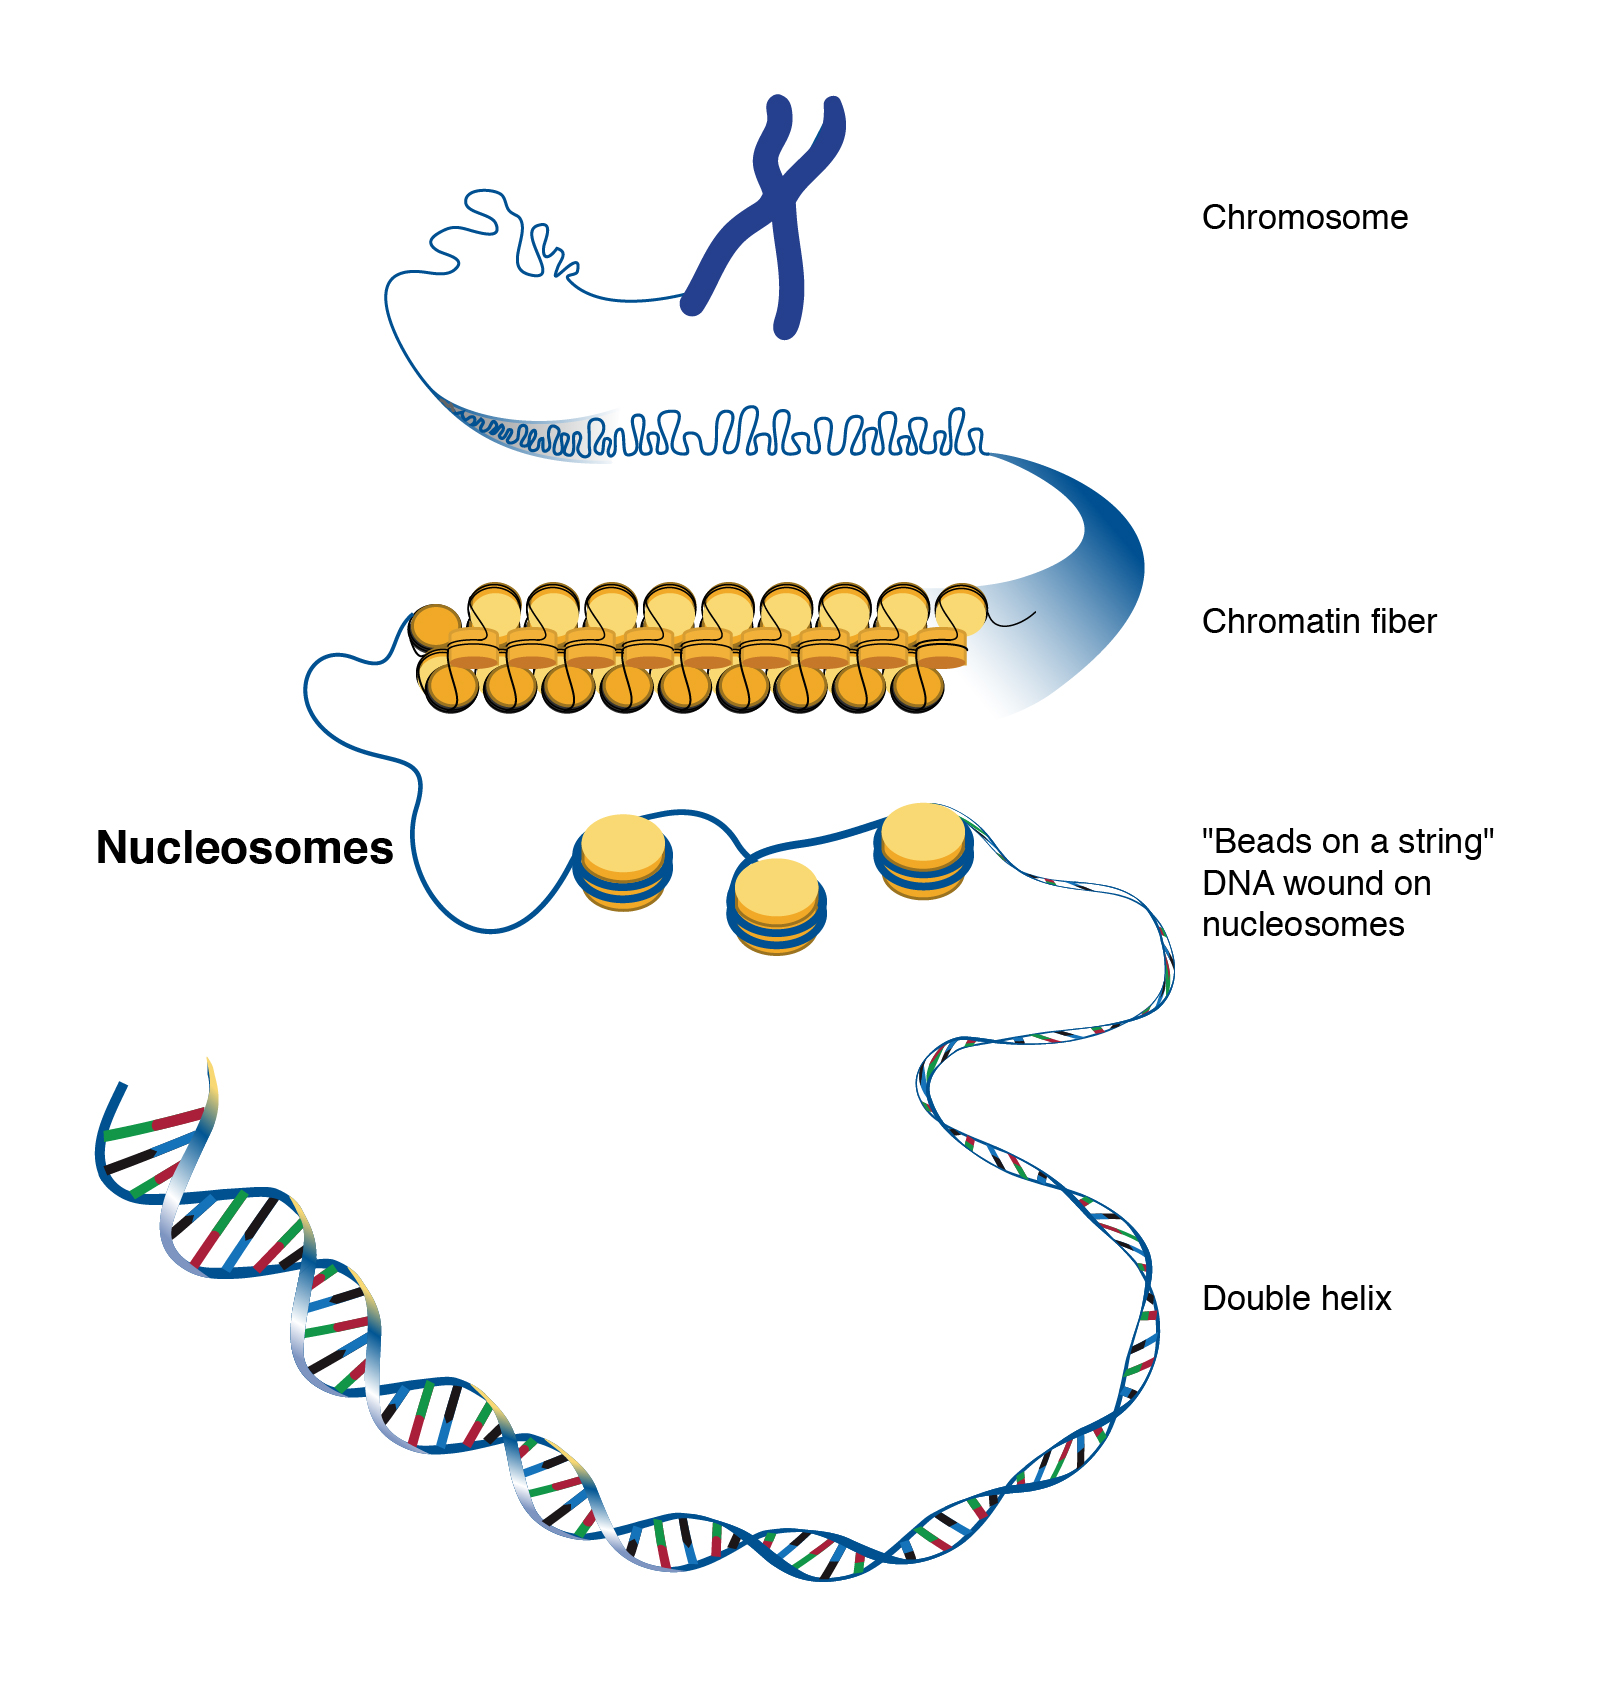
\includegraphics[width=.8\textwidth]{figures/nucleosome1}
	\caption{Organizácia eukaryotického genómu.\label{o:latex_friendly_zone}}
\end{figure}

Nie sú známe žiadne výnimky z tohto vzora: eukaryoty, ktoré boli študované, obsahujú molekuly DNA, ktoré sú vždy lineárne a majú najmenej dva chromozómy. 
Jediná variabilita na tejto úrovni organizácie eukaryotického genómu je zaviazana na počte chromozómov.
Ďalej sa zdá, že biologické vlastnosti organizmu nezávisia od počtu chromozómov \cite{Genomes3}.

Konce eukaryotických chromozómov sú tiež koncami lineárnej duplexnej DNA a ako také si vyžadujú špeciálnu štruktúru, ktorá by zaisťovala ich zachovanie.
Dôvod je spojený so spôsobom, akým sa replikuje dvojvláknová DNA \cite{PrinciplesOfGeneManipulation}.
Ak by neexistoval spôsob dokončovania koncov, chromozómy by sa po každom delení buniek skracovali.

Teloméry sú špecializované sekvencie nukleových kyselín, ktorých úlohou je chrániť konce chromozómov.
Vo väčšine eurkaryotickych buniek pozostáva telomer z krátkeho opakovania nukleotidov TTAGGG s dĺžkou stoviek jednotiek, ale opakovaný segment sa môže medzi jednotlivými druhmi líšiť.
Tieto opakovania sa tiež medzi jednotlivými druhmi značne líšia, avšak každý druh si zachováva fixnú priemernú dĺžku telomerov vo svojej rodovéj línii.

Napriek veľkosti jadra (5 - 10 um) je celková dĺžka DNA v ľudskej bunke približne 2,1 m a môže byť zabalená do bunky vďaka spôsobu, ktorým je nukleová kyselina uložená (obr 1.4).

Genetický materiál vo vírusoch a baktériách pozostáva z reťazcov DNA alebo RNA takmer bez bielkovín.
U eukaryotov je však podstatné množstvo bielkovín ktoré sú spojené s DNA na udržanie štruktúry.
Takýto komplex bielkovín a DNA sa nazýva chromatín.

Na najnižšej úrovni je DNA organizovaná obalením vlákien DNA okolo proteínov nazývaných históny, ktoré obsahujú veľké množstvo pozitívne nabitých aminokyselín arginínu a lyzínu.
Tieto aminokyseliny ako súčasť histónov všeobecne hrajú rozhodujúcu štrukturálnu úlohu, čo umožňuje viazať negatívne nabité fosfátové skupiny nukleotidov.

\begin{figure}[!ht]
	\centering
	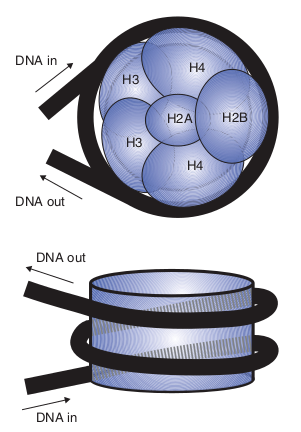
\includegraphics[width=.5\textwidth]{figures/nucleoDetailed}
	\caption{The nucleosome structure. H2A, H2B, H3 and H4 represent different types of histones. \label{o:latex_friendly_zone}}
\end{figure}

V priemere DNA namotaná okolo histónov pozostáva z 140 - 150 párov báz, v závislosti od druhu.
Takýto komplex DNA a histónov sa nazýva nukleozóm (obr. 1.5).
Tieto nukleozómy, ktoré sú súčasťou chromatínu, môžu byť ďalej navíjané do čoraz väčších závitov až do vytvorenia chromozómov.

Tesné navinutie DNA však obmedzuje schopnosť buniek dostať sa k DNA a spracovať ju.
Namiesto toho, aby bola nukleová kyselina neustále zvinutá, nachádza sa zvyčajne v stave zvanom chromatín, kde sú niektoré segmenty kyseliny pevne navinuté (heterochromatín), zatiaľ čo iné segmenty sú úplne otvorené (euchromatín).
Euchromatínová DNA je vysoko dostupná pre molekulárne komplexy používané bunkou, a preto sa s ňou ľahšie manipuluje.

Množstvo a rozsah navinutie DNA určuje bunka, ktorá kontroluje, ktoré časti genómu je možné využivať na syntézu proteinov a ktoré nie.
Toto navinutie DNA vplyvňuje bunkovú funkciu a javí sa ako hlavná príčina diferenciácie typu buniek pri rovnakej DNA.

%%%%%%%%%%%%%%%%%%%%%%%%%%%%%%%%%%%%%%%%%%%%%
\subsection{Organizácia prokaryotického genómu}
%%%%%%%%%%%%%%%%%%%%%%%%%%%%%%%%%%%%%%%%%%%%%
Prokaryot je bunkový organizmus, ktorému chýba obalené jadro.
Prokaryotické genómy sa veľmi líšia od eukaryotických, najmä čo sa týka fyzickej organizácie genómu v bunke.
Aj keď sa slovo „chromozóm“ používa na opis štruktúr DNA a proteínov prítomných v prokaryotických bunkách, jedná sa o nesprávny názov, pretože táto štruktúra nepripomína obyčajný eukaryotický chromozóm.
V typickom prokaryote je genóm obsiahnutý v jedinej kruhovej molekule DNA lokalizovanej v nukleoide - ľahko sa sfarbujúcej oblasti inak nevýraznej prokaryotickej bunky (obr. 1.6).

\begin{figure}[!ht]
	\centering
	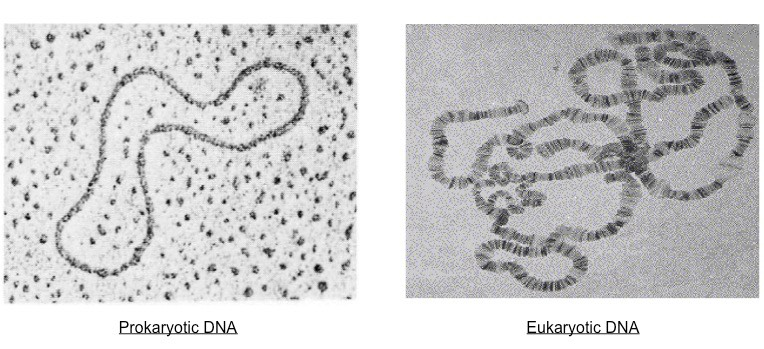
\includegraphics[width=\textwidth]{figures/pro-vs-eu-dna_med.jpeg}
	\caption{Porovnanie eukaryotickej a prokaryotickej DNA.\label{o:latex_friendly_zone}}
\end{figure}

Väčšina toho, čo je známe o organizácii DNA v nukleoide, pochádza zo štúdií \textit{E. coli}.
Prvou rozoznateľnou vlastnosťou, bolo, že kruhový genóm \textit{E. coli} je zvinutý.
Superzávitnica nastáva, keď sa do dvojitej špirály DNA zavedú ďalšie dvojité špirály (pozitívna nadzávitnica) alebo ak sa odstránia závity (negatívna nadzávitnica).
Pri lineárnej molekule sa torzné napätie vyvolané pretočením alebo odtočením okamžite uvoľní rotáciou koncov molekuly DNA, ale kruhová molekula, ktorá nemá konce, nemôže týmto spôsobom uvoľniť napätie.
Namiesto toho kruhová molekula reaguje navinutím okolo seba a vytvorí kompaktnejšiu štruktúru.
Nadzávitnutie je preto ideálny spôsob, ako zabaliť kruhovú molekulu do malého priestoru.

Napriek konvenčnej prokaryotickej štruktúre genómu sa nachádza čoraz viac lineárnych genómov.
Lineárne molekuly majú voľné konce, ktoré musia byť odlíšiteľné od zlomov DNA, takže tieto chromozómy vyžadujú terminálne štruktúry rovnocenné s telomérami eukaryotických chromozómov.
U \textit{Borrelia burgdorferi} a \textit{Agrobacterium tumefaciens} sú skutočné konce chromozómov rozlíšiteľné, pretože sa vytvára kovalentná väzba.
medzi 5` a 3` koncami polynukleotidov v dvojitej špirále DNA a v Streptomyces coelicolor sa konce zdajú byť označené špeciálnymi väzbovými proteínmi.

%%%%%%%%%%%%%%%%%%%%%%%%%%%%%%%%%%%%%%%%%
\subsection{Organizácia vírusových genómov}
%%%%%%%%%%%%%%%%%%%%%%%%%%%%%%%%%%%%%%%%%

V prvom rade sú vírusy mimobunkovou formou života. To znamená, že ich životný cyklus a štruktúra sú vo všeobecnosti menej komplikované v porovnaní s ostatnými.
Vírusy môžu mať extrémne jednoduchý dizajn, ktorý sa skladá z nukleovej kyseliny obklopenej proteínovým obalom známym ako kapsida (obr 1.7).
Kapsida je zložená z menších bielkovinových zložiek, ktoré sa označujú ako kapsoméry. Kombinácia kapsid + genóm sa nazýva nukleokapsid.

\begin{figure}[!ht]
	\centering
	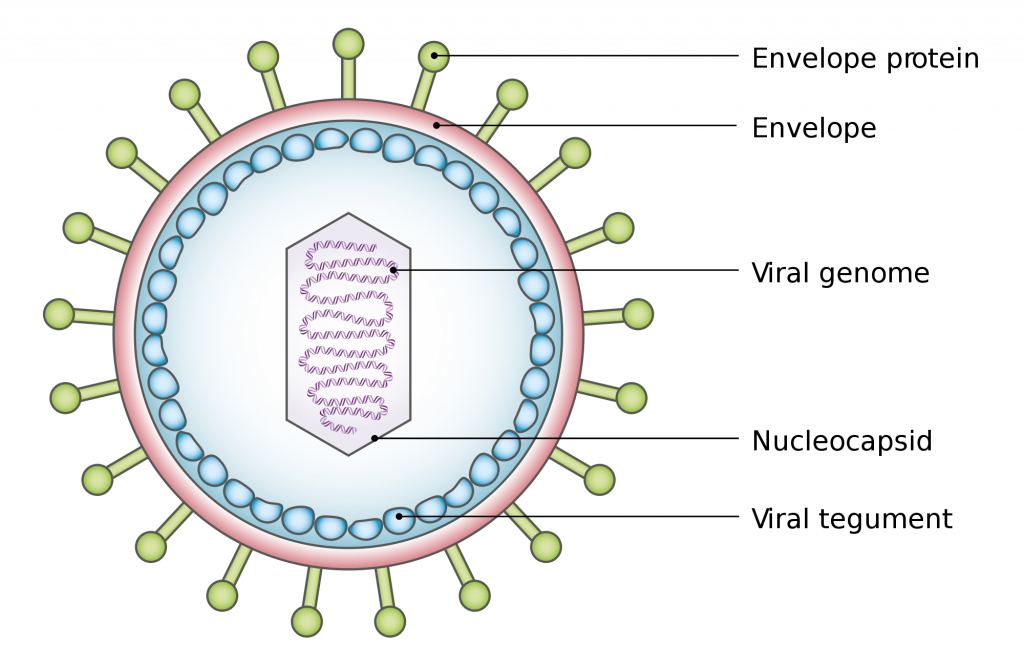
\includegraphics[width=.75\textwidth]{figures/virus.png}
	\caption{Charakteristika vírusu \label{o:latex_friendly_zone}}
\end{figure}

Vírusy môžu obsahovať aj ďalšie zložky, pričom najbežnejšou je ďalšia membránová vrstva obklopujúca nukleokapsid, ktorá sa nazýva obálka.
Obal sa skutočne získava z jadrovej alebo plazmatickej membrány infikovanej hostiteľskej bunky a potom sa modifikuje vírusovými proteínmi nazývanými peploméry.
Niektoré vírusy obsahujú vírusové enzýmy, ktoré sú potrebné na infekciu hostiteľskej bunky a sú kódované vo vírusovom genóme.
Kompletný vírus so všetkými zložkami potrebnými na infekciu hostiteľských buniek sa označuje ako virión.

Zatiaľ čo bunky obsahujú pre svoj genóm dvojvláknovú DNA, vírusy sa neobmedzujú iba na túto formu.
Navyše, ako bolo uvedené na samom začiatku, okrem vírusov dsDNA (dvojvláknová DNA) existujú aj vírusy s jednovláknovou DNA (ssDNA), dvojvláknovou RNA (dsRNA) a jednovláknovou RNA (ssRNA).
V tejto poslednej kategórii môže byť ssRNA buď pozitívna v zmysle (+ ssRNA, čo znamená, že môže prepisovať správu, napríklad mRNA), alebo môže byť v negatívnom zmysle (-ssRNA, čo naznačuje, že je komplementárna k mRNA). Niektoré vírusy dokonca začínajú jednou formou nukleovej kyseliny v nukleokapside a potom ju počas replikácie konvertujú do inej formy.
Môžu byť navyše viacdielne, čo znamená, že pozostávajú z niekoľkých molekúl RNA.

Všeobecne DNA vírusy majú väčšiu veľkosť ako RNA vírusy a jednovláknové genómy sú menšie ako dvojvláknové.
Existuje hypotéza, že jednovláknový vírus je menší, pretože tento typ molekuly je krehkejší ako dvojvláknová molekula.
To všeobecne platí pre vírusy ssDNA aj ssRNA.
Medzi dvojvláknovými genómami môžu mať buď „malé“, alebo „veľké“ genómy.
Jedným z hlavných rozdielov medzi týmito dvoma genómami je mechanizmus replikácie DNA.
Malé genómy využívajú aktivity hostiteľskej polymerázy, zatiaľ čo veľké genómy kódujú vlastnú DNA polymerázu.

%%%%%%%%%%%%%%%%%%%%%%%%%%%%%%%%%%%%%%%%%%%%%%%%%%%
\subsection{Gény: umiestnenie a všeobecná štruktúra}
%%%%%%%%%%%%%%%%%%%%%%%%%%%%%%%%%%%%%%%%%%%%%%%%%%%
Gén je sekvencia nukleotidov v DNA alebo RNA, ktorá kóduje syntézu génového produktu, buď RNA alebo proteínu, ktoré majú charakteristické vlastnosti.
Povaha všetkých týchto špecifických znakov nie je v súčasnosti úplne pochopiteľná, a preto kontrola sekvencie nie je spoľahlivým spôsobom lokalizácie génov \cite{Genomes3}.

Okrem obvyklých génov sú aj pseudogény prítomné v rôznych genómoch.
Pseudogény sú sekvencie genómovej DNA s takou podobnosťou s normálnymi génmi, že sa považujú za nefunkčné kópie alebo za blízkych príbuzných génov \cite{PrinciplesOfGeneManipulation}. 
Sú tvorené dvoma spôsobmi:
\begin{itemize}
	\item Klasické duplikované pseudogény sa tvoria, keď tandemovo duplikované gény akumulujú mutácie tak, že jeden z génov sa stane nefunkčným.
	Tieto mutácie môžu zabrániť transkripcii a / alebo translácii (procesy potrebné pre syntézu proteínov).
	\item Spracované pseudogény sa tvoria hromadením mutácií v géne, ktorý bol retrotransponovaný na nové miesto.
	Vyznačujú sa absenciou intrónov (vid' d'alej), ktoré sú prítomné v rodičovskom géne.
\end{itemize} 

Gény, ktoré kódujú proteíny, zahŕňajú otvorené čítacie rámce (ORF) pozostávajúce zo série kodónov (trinukleotidov), ktoré špecifikujú aminokyselinovú sekvenciu proteínu, ktorý gén kóduje.
ORF začína iniciačným kodónom - zvyčajne (ale nie vždy) ATG - a končí terminačným kodónom: TAA, TAG alebo TGA.
Hľadanie DNA sekvencie pre ORF, ktoré začínajú ATG a končia terminačným tripletom, je preto jedným zo spôsobov hľadania génov.
Analýzu komplikuje skutočnosť, že každá sekvencia DNA má na komplementárnom vlákne šesť čítacích rámcov, tri v jednom smere a tri v opačnom smere (obr. 1.8).

\begin{figure}[!ht]
	\centering
	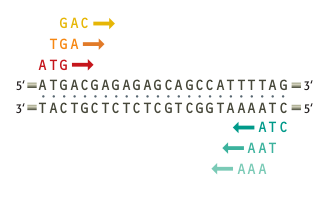
\includegraphics[width=.6\textwidth]{figures/ORF2.png}
	\caption{Both
	strands are read in the 5`3`direction. Each
	strand has three reading frames, depending
	on which nucleotide is chosen as the
	starting position.\label{o:latex_friendly_zone}}
\end{figure}

Kľúčom k úspechu skenovania ORF je frekvencia, s akou sa v sekvencii DNA objavujú terminačné kodóny.
Ak má DNA náhodnú sekvenciu a obsah GC 50\%, potom sa každý z troch terminačných kodónov - TAA, TAG a TGA - objaví v priemere raz za 64 bp.
Ak je obsah GC vyšší ako 50\%, potom sa terminačné kodóny, ktoré sú bohaté na AT, vyskytujú menej často, ale stále sa bude očakávať jeden za každých 100–200 bp.
To znamená, že náhodná DNA by nemala vykazovať veľa ORF dlhších ako 50 kodónov \cite{orf}.
Väčšina génov je naopak dlhšia ako 50 kodónov: priemerná dĺžka je 317 kodónov pre \textit{Escherichia coli}, 483 kodónov pre Saccharomyces cerevisiae a približne 450 kodónov pre človeka \cite{FindingGenes}.
Skenovanie ORF vo svojej najjednoduchšej forme preto berie údaj, napríklad 100 kodónov, ako najkratšiu dĺžku predpokladaného génu a zaznamenáva pozitívne zásahy do všetkých ORF dlhších ako je táto.
With bacterial genomes, simple ORF scanning is an effective way of locating most of the genes in a DNA sequence.
The real genes in the sequence cannot be mistaken because they are much longer than 50 codons in length. 
With bacteria the analysis is further simplified by the fact that the genes are very closely spaced and hence there is relatively little intergenic DNA in the genome (only 11\% for \textit{E. coli}). 
The most of bacterial genes do not overlap.

\begin{figure}[!ht]
	\centering
	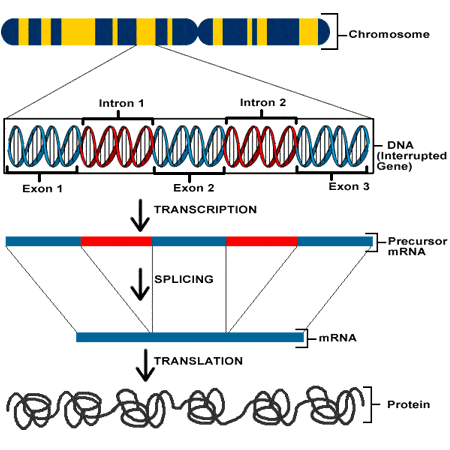
\includegraphics[width=.6\textwidth]{figures/eukaryotic_transcription_2.png}
	\caption{Organizácia intrónov a exónov počas procesov koherentných s DNA v životnom cykle bunky.\label{o:latex_friendly_zone}}
\end{figure}
Aj keď skenovanie ORF funguje dobre pre bakteriálne genómy, je menej efektívne pri lokalizácii génov v sekvenciách DNA od vyšších eukaryotov.
Je to čiastočne preto, že medzi skutočnými génmi v eukaryotickom genóme je podstatne viac priestoru (napríklad približne 62\% ľudského genómu je intergénnych), čo zvyšuje šance na nájdenie falošných ORF.
Ale hlavným problémom ľudského genómu a genómov vyšších eukaryotov všeobecne je, že ich gény sú často štiepené intrónmi (nekódujúce oblasti génu), a tak sa v sekvencii DNA nejavia ako spojité ORF.
Mnoho exónov (kódujúcich oblastí génu) sú kratšíe ako 100 kodónov, niektoré pozostávajú z menej ako 50 kodónov a pokračovanie čítacieho rámca do intrónu zvyčajne vedie k terminačnej sekvencii, ktorá sa zdá uzavrieť ORF (obr. 1.9).
Inými slovami, gény vyššieho eukaryotu sa neobjavujú v sekvencii genómu, pokiaľ sú dlhé ORF a jednoduché skenovanie ORF ich nedokáže lokalizovať.

Navyše, keďže niektoré vírusy (hlavne eukaryotické) majú vo svojich genómoch štruktúry intrón-exón \cite{Genes3}, skenovanie ORF nie je nezvratnou metódou lokalizácie génov medzi nimi.

Skenovanie ORF je vhodné pre gény kódujúce proteín, ale gény pre funkčné RNA, ako sú rRNA a tRNA, neobsahujú otvorené čítacie rámce.
Funkčné molekuly RNA však majú svoje vlastné charakteristické znaky, ktoré môžu byť použité na uľahčenie ich objavenia v sekvencii genómu (obr. 1.10).

\begin{figure}[!ht]
	\centering
	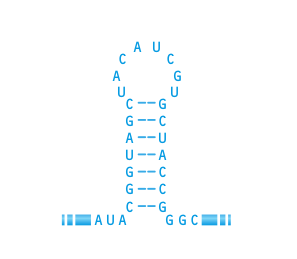
\includegraphics[width=.5\textwidth]{figures/rna.png}
	\caption{Typická štruktúra párovania intramolekulárnych báz RNA.\label{o:latex_friendly_zone}}
\end{figure}

Najdôležitejšou z týchto vlastností je schopnosť zložiť sa do sekundárnej štruktúry, ako je napríklad štvorlístok prijatý molekulami tRNA.
Tieto sekundárne štruktúry sú držané spolu párovaním báz nie medzi dvoma samostatnými polynukleotidmi, ako napríklad v dvojitej špirále DNA,
ale medzi rôznymi časťami toho istého polynukleotidu - párovanie intramolekulárnych báz.

Aby sa mohli vytvoriť intramolekulárne páry báz, musia byť nukleotidové sekvencie v dvoch častiach molekuly komplementárne,
a na vytvorenie komplexnej štruktúry, ako je štvorlístok, musia byť komponenty týchto párov komplementárnych sekvencií usporiadané v charakteristickom poradí v rámci sekvencie RNA.
Tieto vlastnosti poskytujú množstvo informácií, ktoré možno použiť na lokalizáciu génov tRNA v sekvencii genómu. 

Rovnako ako tRNA, rRNA a niektoré z malých funkčných RNA tiež prijímajú sekundárne štruktúry, ktoré sú dostatočne zložité na to, aby umožnili identifikáciu ich génov bez veľkých ťažkostí \cite{rna}.
Menej ľahko sa dajú lokalizovať ďalšie funkčné gény RNA, pretože RNA zaberajú štruktúry, ktoré zahŕňajú relatívne malé párovanie báz alebo párovanie báz nie je v pravidelnom obrazci.

\bigskip
\smallskip

Na zhrnutie, je môžne vyvodiť závery o tom, ako presne je možné zobraziť štruktúru genómu SARS-CoV-2, a to, že najjednoduchšie vizualizácie sa môžu týkať nasledujúcich oblastí:
\begin{itemize}
	\item Vizualizácia nukleotidovej sekvencie za účelom vyhľadávania vzorov a vyhodnotenia ich štatistickej distribúcie v reťazci DNA.
	\item Vizualizácia pozícií génov s cieľom analyzovať oblasti genómu, ktoré kódujú určité proteíny.
	\item Vizualizácia pozícií intrónov a exónov ak sa ide o genómy eukaryotov.
\end{itemize} 

%%%%%%%%%%%%%%%%%%%%%%%%%%%%%%%%%%%%%%%%%%%%%%%%%%%%%%%%%%
\section{Existujúce riešenia pre reprezentáciu údajov o genóme}
%%%%%%%%%%%%%%%%%%%%%%%%%%%%%%%%%%%%%%%%%%%%%%%%%%%%%%%%%%
Vďaka rýchlemu vývoju technológií sekvenovania novej generácie sa sekvenovali státisíce genómov.
Všetky údaje o postupnosti, ako aj anotácie sa zhromažďujú v databázach genómu a sú verejne dostupné
prostredníctvom webových portálov, ako je portál genómov NCBI a webová stránka databázy genómov EBI. %(http://www.ncbi.nlm.nih.gov/genome/) (http://www.ebi.ac.uk/Databases/genomes.html)

Systematickou integráciou sekvencií genómu spolu s anotáciami generovanými prostredníctvom mnohých heterogénnych údajov, prehliadač genómu poskytuje jedinečnú platformu pre molekulárnych biológov, aby mohli tieto genomické údaje efektívne a pohodlne prehliadať, vyhľadávať, získavať a analyzovať.
Vďaka grafickému rozhraniu pomáha prehliadač genómu používateľom intuitívne extrahovať a sumarizovať informácie z obrovského množstva nespracovaných komplexných údajov.

Prehliadače genómu možno vo všeobecnosti rozdeliť na webové prehľadávače a samostatné aplikácie.
Webové prehliadače genómu, ktoré sú zvyčajne vhodnejšie na podporu biologického výskumu vďaka svojej kvalite údajov, flexibilnej dostupnosti a vysokému výkonu.
\begin{itemize}
	\item Po prvé, špecializované organizácie často zhromažďujú a integrujú vysoko kvalitné anotačné údaje do webových prehľadávačov genómu a poskytujú komunite množstvo aktuálnych informácií. 
	\item Po druhé, používatelia k nim môžu mať prístup kdekoľvek pomocou štandardného webového prehľadávača, čím sa vyhnú ďalšiemu úsiliu pri nastavovaní lokálneho prostredia pre inštaláciu aplikácií a prípravu dát. 
	\item Po tretie, webové prehľadávače genómu sa zvyčajne inštalujú na vysoko výkonné servery a môžu podporovať zložitejšie a rozsiahlejšie dátové typy a aplikácie.
\end{itemize}

%%%%%%%%%%%%%%%%%%%%%%%%%%%%%%%%%%%%%%%
\subsection{Webové prehliadače genómu}
%%%%%%%%%%%%%%%%%%%%%%%%%%%%%%%%%%%%%%%

V súčasnosti existujú dva typy webových prehľadávačov genómu. 

Prvým typom sú prehliadače genómu pre viac druhov, ako napríklad projekt Ensembl \cite{ENSEMBLgb}, databáza genómov UCSC \cite{UCSCgb} a webová stránka prehliadača NCBI \cite{NCBIgb}.
Tieto prehľadávače genómu podporujú medzidruhovú komparatívnu analýzu.
Väčšina z nich obsahuje veľké množstvo anotácií, ktoré zahŕňajú génový model, dôkazy o transkripcii, profily expresie, regulačné údaje, genómovú konverzáciu atď.
Každá skupina vopred vypočítaných údajov anotácií sa v prehľadávačoch genómu nazýva stopa.
Podstatou prehliadača genómu je zhromaždiť viac stôp pod rovnakou genomickou súradnicou pozdĺž osi Y, aby používatelia mohli ľahko preskúmať konzistenciu alebo rozdielnosť anotačných údajov a urobiť úsudok o vlastnostiach genomickej oblasti.

Druhým typom sú druhovo špecifické prehliadače genómu, ktoré sa zameriavajú hlavne na jeden modelový organizmus a môžu mať pre konkrétny druh viac anotácií.
Poháňaný projektom Generic Model Organism Database (GMOD) sa zhromažďujú desiatky softvérových nástrojov otvoreného zdroja na vytváranie a správu biologických databáz genómu.
Rámec GBrowse \cite{GBrowse} je jedným z najpopulárnejších nástrojov v projekte GMOD.
Tabuľka 1.2 uvádza zoznam niekoľkých bežných webových prehľadávačov genómu, medzi ktoré patrí Ensembl, prehľadávač genómov UCSC a GBrowse, ku ktorým má prístup veľké množstvo používateľov na celom svete.

%%%%%%%%%%%%%%%%%%%%%%%%%%%%%%%%%%%%%%%%%%
\subsection{Funkcie a vlastnosti}
%%%%%%%%%%%%%%%%%%%%%%%%%%%%%%%%%%%%%%%%%%

Webový prehliadač genómu často poskytuje centralizovanú databázu alebo súbor databáz na ukladanie rôznych typov anotačných údajov získaných od niekoľkých organizácií.
Výzvou pre všeobecné prehľadávače genómu je, ako správne zobraziť tieto informácie pre rôzne stupne genómu.
Keď je požadovaná veľká genomická oblasť, je potrebné do obrazu zahrnúť obrovské množstvo informácií, ktoré by mohli preťažiť server a sieť.
Príliš veľa ťažkých a komplikovaných detailov navyše narúša pozornosť používateľa.

\begin{figure}[!ht]
	\centering
	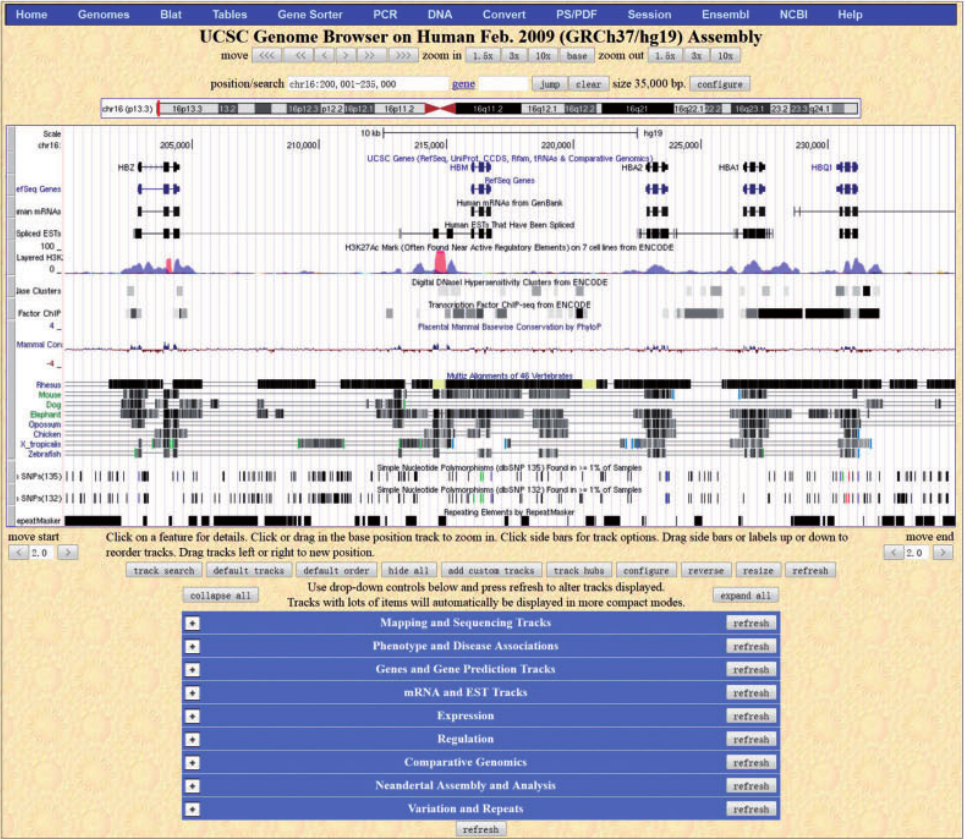
\includegraphics[width=.9\textwidth]{figures/ucsc_gb.png}
	\caption{Hlavné používateľské rozhranie prehľadávača genómov UCSC, ktoré zobrazuje predvolené stopy v predvolenom poradí pre klaster ľudského génu alfa-globínu.\label{o:latex_friendly_zone}}
\end{figure}

Prehliadač genómu UCSC, ktorý je jedným z veľkých hráčov vo vizualizácii genomických údajov, sa snaží tento problém vyriešiť poskytnutím viacerých zobrazení tracku (obr. 1.11).
Každú stopu je možné zobraziť v rôznych režimoch, napríklad hustú, úplne rozbalenú alebo skrytú.
Používateľ môže ísť hlbšie po hustej trati 25 a otvoriť ju v plnom režime.
Pre zobrazenie tracku je možné veľa stupníc.
Najnižší je jeden chromozóm a najvyššia stupnica je sekvencia párov báz.
Môže sa zobraziť hustý pohľad na niektoré tracky, aby sa pri oddialení na veľkú oblasť chromozómu skryli komplikované detaily, aby mal používateľ široký obraz o vybranej oblasti chromozómov.

\begin{figure}[!ht]
	\centering
	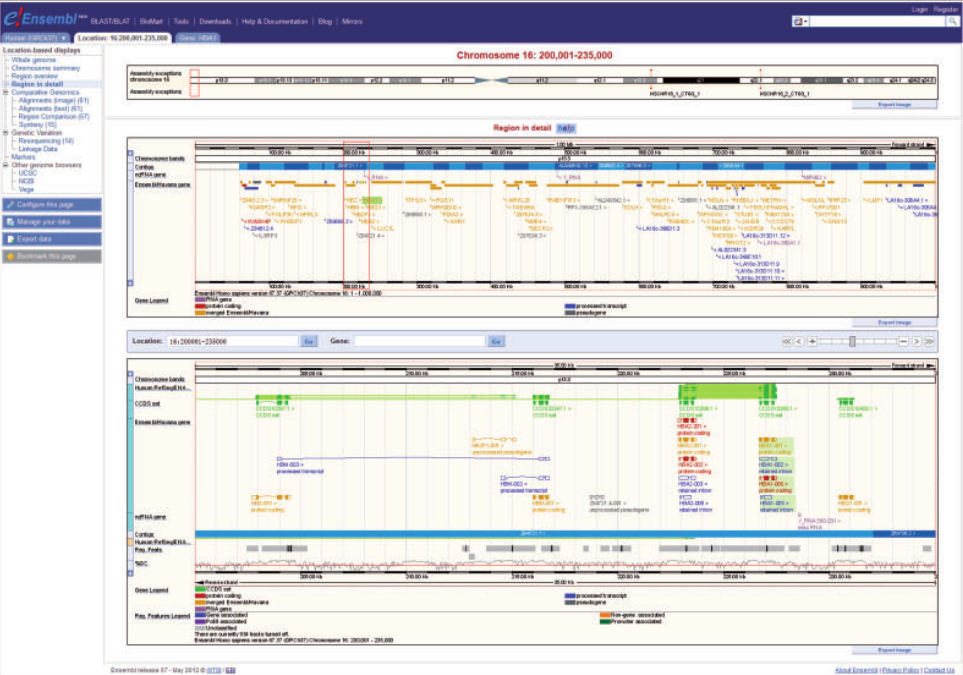
\includegraphics[width=.9\textwidth]{figures/ensembl_gb.png}
	\caption{Užívateľské rozhranie prehliadača genómu Ensembl s predvoleným nastavením stôp anotácií zobrazujúcich klaster génov alfa-globínu. Grafické anotácie sú zobrazené v hlavnej časti tela rozdelené do troch sekcií zhora nadol.\label{o:latex_friendly_zone}}
\end{figure}

Prehliadač genómu Ensembl poskytuje rovnaké užívateľské rozhranie pre každý organizmus.
Hlavné telo rozhrania obsahuje dva panely (obr. 1.12).

Na ľavom paneli je uvedená hlavná ponuka pre zobrazenia založené na polohe na rôznych úrovniach od celého genómu, súhrnu chromozómov až po prehľad oblastí a podrobných oblastí.
Poskytnuté sú tiež odkazy na komparatívnu genomiku, genetické variácie a sekvenčné markery.
Hlavný panel je usporiadaný do troch častí zhora nadol a poskytuje používateľom rôzne stupnice na analýzu genómu.
Okrem zobrazenia umiestnenia poskytuje Ensembl samostatné stránky na zobrazenie rôznych typov informácií usporiadaných do štruktúr so záložkami.
Je užitočné mať prehľad o veľkej ploche chromozómu a súčasne hľadať podrobnosti do niekoľkých malých oblastí.
Spojenie paralogických génov na jednej stránke by mohlo výrazne podporiť komparatívnu analýzu.

Napríklad prehliadač sekvencií NCBI podporuje používateľov pri prezeraní rôznych oblastí vo vnútri toho istého chromozómu a poskytuje flexibilný navigačný prístup založený na viacerých paneloch s rôznymi farebnými kurzormi označujúcimi príslušné genómové polohy.

Ako už bolo spomenuté vyššie, existujú druhovo špecifické prehliadače genómu, ktoré sú k dispozícii online.
Svetlým príkladom takýchto nástrojov je prehliadač genómu ryže MSU a prehliadač genómu Rice-Map \cite{RMgb}.

\begin{table}[]

	\caption{Hlavné funkcie populánych prehľadávačov genómu. BioMart a BioDas sú komunitné projekty, ktoré poskytuju jediný prístupový bod k distribuovaným výskumným údajom}\label{t:1}
	\smallskip
	\centering

	\begin{tabular}{|l|l|l|c|}
	\hline
	\multicolumn{1}{|c|}{\textbf{Vlastnosti}}                              & \multicolumn{1}{c|}{\textbf{UCSC}}                                               & \multicolumn{1}{c|}{\textbf{Ensemble}}                                                            & \textbf{GBrowse}                                                                                           \\ \hline
	\multicolumn{4}{|c|}{Vizualizácia}                                                                                                                                                                                                                                                                                                                                      \\ \hline
	\begin{tabular}[c]{@{}l@{}}Anotácia \\ navigácia\end{tabular}     & \begin{tabular}[c]{@{}l@{}}Prehliadanie\\ podľa stránok, \\ umožňujúce\\ pretiahnutie\end{tabular} & \begin{tabular}[c]{@{}l@{}}Prehliadanie\\ podľa stránok\end{tabular}                                     & \multicolumn{1}{l|}{\begin{tabular}[c]{@{}l@{}}Prehliadanie\\ podobné mape\\ v obmedzenom\\ regióne \\\end{tabular}} \\ \hline
	\begin{tabular}[c]{@{}l@{}}Viaceré okná\\ na stránke\end{tabular}   & \multicolumn{1}{c|}{-}                                                           & \multicolumn{1}{c|}{-}                                                                            & -                                                                                                          \\ \hline
	\multicolumn{4}{|c|}{Získavanie a analýza údajov}                                                                                                                                                                                                                                                                                                                        \\ \hline
	Systém dopytov                                                         & Prehliadač tabuliek                                                                    & BioMart                                                                                           & -                                                                                                          \\ \hline
	\begin{tabular}[c]{@{}l@{}}Užívateľsky\\ orientovaná \\ analýza\end{tabular}    & \begin{tabular}[c]{@{}l@{}}Priame\\ odoslanie\\ údajov\end{tabular}                & \multicolumn{1}{c|}{-}                                                                            & \multicolumn{1}{l|}{\shortstack{Doplnkové \\ nástroje}}                                                                          \\ \hline
	\begin{tabular}[c]{@{}l@{}}Strojovo\\ orientované \\ rozhranie\end{tabular} & \multicolumn{1}{c|}{-}                                                           & \begin{tabular}[c]{@{}l@{}}\shortstack{Prostredníctvom \\ BioMart}\end{tabular}                                         & \multicolumn{1}{l|}{\shortstack{Prostredníctvom \\ BioDAS}}                                                                        \\ \hline
	\multicolumn{4}{|c|}{Prispôsobenie}                                                                                                                                                                                                                                                                                                                                      \\ \hline
	\shortstack{Nahrajte stopy\\používateľov}                                                  & \multicolumn{1}{c|}{+}                                                           & \multicolumn{1}{c|}{+}                                                                            & +                                                                                                          \\ \hline
	\begin{tabular}[c]{@{}l@{}}Obsah \\prispievaný\\ používateľmi\end{tabular}  & \begin{tabular}[c]{@{}l@{}}Obnovenie dát\\na základe relácie\end{tabular}           & \begin{tabular}[c]{@{}l@{}}Mechanizmus osobnej \\ anotácie, \\ záložky \\ a skupiny\end{tabular} & -                                                                                                          \\ \hline
	\end{tabular}
\end{table}

V prehliadači genómu ryže MSU môžu používatelia prehľadávať gén OsSPL14 zadaním výrazu „SPL14“ do vyhľadávacieho poľa.
Prehliadač genómu ryže MSU, ktorý je založený na platforme GBrowse, poskytuje anotačné pohľady v rôznych mierkach, vrátane prehľadu chromozómov, regionálneho a podrobného zobrazenia (obr. 1.13).

\begin{figure}[!ht]
	\centering
	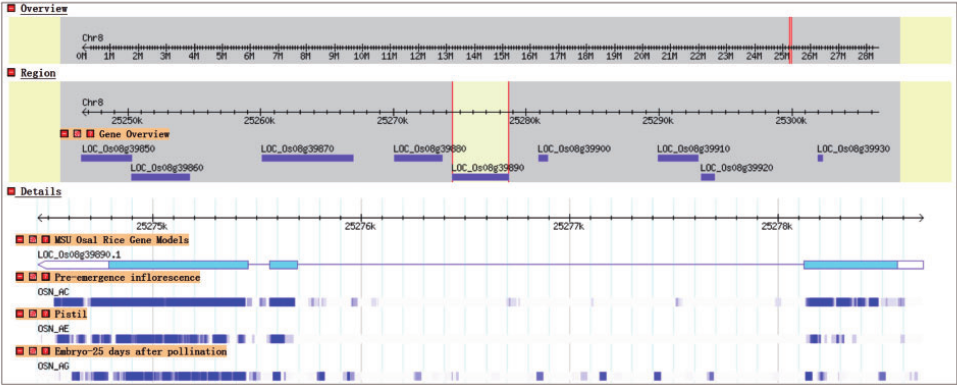
\includegraphics[width=.9\textwidth]{figures/ss-1.png}
	\caption{Užívateľské rozhranie prehliadača genómu ryže MSU. Prehľad chromozómov je zobrazený v hornej časti, regionálne zobrazenie je zobrazené v strede a spodná časť predstavuje podrobné zobrazenie pre štyri stopy anotácií.\label{o:latex_friendly_zone}}
\end{figure} 

Zväčšené zobrazenie poskytuje používateľom širší obraz, aby mohli pohodlne skontrolovať anotáciu pred a za.
Na podrobnom anotačnom plátne je poskytnutých viac ako 82 anotačných stôp, ktoré zahŕňajú génový model, dôkaz transkriptu, profilovanie expresie, zarovnanie sekvencie, genetický marker, SNP, pokrytie RNA-Seq a ďalšie genómové znaky.
Okrem základných informácií o génovom modeli môžu používatelia skontrolovať tento gén v rôznych vývojových štádiách prostredníctvom rôznych expresných údajov RNA-Seq.

V prehľadávači genómu Rice-Map sú rôzne stopy anotácií usporiadané do vizualizačného plátna podobného mape, pričom názov otvorených stôp je uvedený na pravom paneli (obr. 1.14).
Okrem základných anotácií génov existujú aj bohaté anotácie pre zosúladenie krížových genómov a hodnoty ochrany, ktoré poskytujú dôležité stopy pre vyšetrovanie tohto génu v iných rastlinách.

\begin{figure}[!ht]
	\centering
	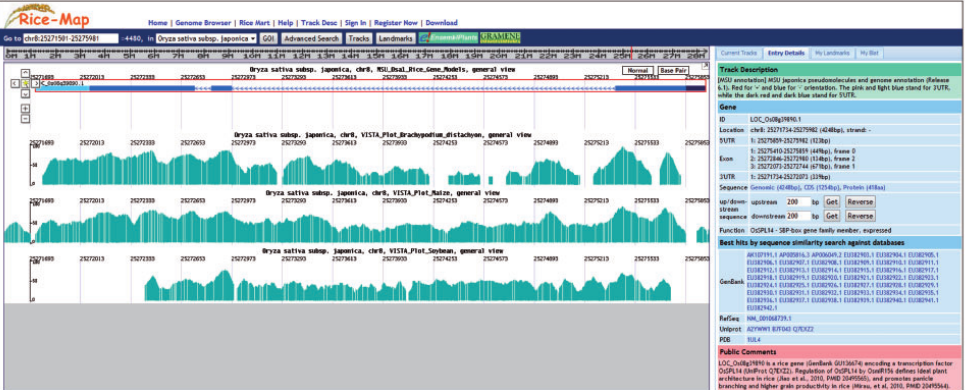
\includegraphics[width=.9\textwidth]{figures/ss-2.png}
	\caption{Prehliadač genómu Rice-Map. Podrobné informácie o jednotlivých položkách sa zobrazujú na pravom paneli a interpretujú zdroj údajov, umiestnenie záznamu, postupnosť a funkciu atď.\label{o:latex_friendly_zone}}
\end{figure}

Pretože prehliadače genómu sú schopné poskytnúť používateľovi množstvo rôznych biologicky špecifických informácií, definícia týchto pojmov nie je uvedená v tejto práci.

\bigskip
\smallskip

Na zhrnutie vykonaéj analýzu, je možné dospieť k záveru, že moderné a populárne nástroje na vizualizáciu genómu majú tendenciu byť zložité, založené na webe a už poskytujú používateľovi všetky potrebné informácie.

Preto, vývoj softvéru zameraného na vizualizáciu 2D genómu bude zameraný na poskytnutie samostatnej konzolovej aplikácie pre používateľa, ktorá využíva niektoré z menej používaných vizualizačných metód.
Kvôli tomu, že SARS-CoV-2 vlastní virusový genóm, vizualizácia bude zameraná len na zobrazenie sekvencií nukleotidov a pozícií ORF.